%PRESTAR ATENCION: pegado de archivo externo!!!

%ARCHIVO transmitir.tex modificado.

%Dada la motivación, se puede decir a priori que el objetivo del presente trabajo es la implementación de una efectiva comunicación entre una Computadora Personal (PC) y una FPGA. Sin embargo, este objetivo tan amplio se plasmará de forma más concreta y detallada en la Sección \ref{int:obj}.\\

El estándar más exigente de la norma americana de la SCTE (Sociedad de Ingenieros de Comunicación por Cable) utilizada Televisión Digital, posee una tasa de \SI{38.8}{\mega\bit\per\second}\cite{SocietyofCableTelecommuniocationsEngineers2006}. Por su parte, la serie de sensores para adquirir imágenes monocromáticas MT9M001, comercializado por ON Semiconductors posee 1280x1024 pixeles, con profundidad de 10 bits y puede operar hasta a 30 cuadros por segundo\cite{MicronTechnology2004}. La tasa de transmisión necesaria es, por tanto, de \SI{393.2}{\mega\bit\per\second}.%\\
%¿Y cuál es el protocolo que mejor se ajusta a la necesidad de disponibilidad? 

Un requerimiento que posee cualquier periférico informático es el de compatibilidad. No es conveniente utilizar puertos que requieran acceso a la placa madre, como el caso de tarjetas de tipo PCI o PCI express, debido a que no todos los equipos los tienen accesible, como ser computadoras portátiles, y en algunos casos estos pueden estar todos ocupados. Se opta, entonces, por alguno de los tres puertos de moda: Ethernet, dedicado principalmente a conexión de redes mediante cables; Wi-Fi, utilizado para el accesos a la red de forma inalámbrica; y USB, dirigido a la comunicación de periféricos con la PC.%\\
%Además, pensando en que la implementación sea compatible con equipos informáticos convencionales, es decir, se encuentren fácilmente en el mercado y no posean especificaciones que escapen al uso de oficina. Esto se cumple hoy en día con tres tipos de puertos: Ethernet, dedicado principalmente a conexión de redes mediante cables; Wi-Fi, utilizado para el accesos a la red de forma inalámbrica; y USB, dirigido a la comunicación de periféricos con la PC.\\

Al hablar de Ethernet o Wi-Fi, se hace referencia a dos formas diferentes de conectarse a una red de computadoras. En otras palabras, se habla de dos o más nodos, compuestos por PCs o cualquier dispositivo electrónico con capacidad de realizar cálculo binario, que pueden intercambiar datos a través de una trama bastante compleja de componentes diferentes. Ambos protocolos hacen referencia solo a la conexión física de los dispositivos y el control de acceso de cada uno de ellos a la conexión. Quedando a cargo de otros sistemas, con sus protocolos, que los datos enviados puedan ser correctamente recibidos por el usuario de la PC. La gran diferencia entre ellos radica en el medio físico que utilizan: Wi-Fi emplea ondas electromagnéticas emitidas mediante radiofrecuencia, mientras que en Ethernet, estas ondas son acarreadas por uno o más conductores, como ser cable coaxial, cables de par trenzado o fibra óptica.%\\

\begin{figure}
	\centering
	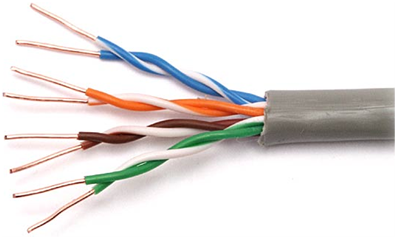
\includegraphics[width=0.4\textwidth]{partrenzado.png}
	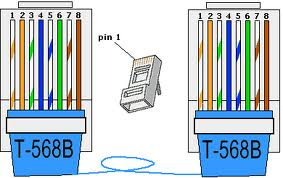
\includegraphics[width=0.4\textwidth]{utp.jpeg}
	\caption{Par Trenzado y un dibujo de su ficha de conexión.}
	\label{fig:utp}
\end{figure}

Ethernet, también conocido como IEEE 802.3, es una norma que define cómo se deben conectar nodos a través de conductores para conformar redes de área local (LAN o {\it Local Area Network}), es decir, redes pequeñas, como ser domésticas, de oficinas o de pequeñas empresas, de forma que puedan transmitir información a velocidades seleccionables entre \SI{1}{\mega\bit\slash\second} y \SI{400}{\giga\bit\slash\second} \cite{Ethernet2018}. Utiliza una tecnología denominada Acceso Múltiple Sensando la Portadora con Detección de Colisiones (CSMA/CD del inglés {\it Carrier Sense Multiple Access with Collision Detection}). En una red con CSMA/CD, cada dispositivo debe sensar en forma permanente la conexión a la red, es decir, no existe un dispositivo que dirija el uso del bus, sino que cada uno debe identificar el estado de la red. Los mensajes se envían modulados. Cuando una señal portadora es detectada, todos chequean la dirección del paquete de información que viaja y el mensaje es recibido solamente por el dispositivo que se corresponda con esa dirección. Siempre que exista una señal portadora en el bus, los dispositivos que deseen transmitir información deberán esperar a fin de evitar colisiones, o sea, que dos dispositivos envíen mensajes a la vez y estos se interfieran.%\\

%Ethernet, también conocido como IEEE 802.3, es una norma que define cómo se deben conectar nodos a través de conductores para conformar redes de área local (LAN o {\it Local Area Network}), es decir, redes pequeñas, como ser domésticas, de oficinas o de pequeñas empresas, de forma que puedan transmitir información a velocidades seleccionables entre \SI{1}{\mega\bit\slash\second} y \SI{400}{\giga\bit\slash\second} \cite{Ethernet2018}. Utiliza una tecnología denominada Acceso Múltiple Sensando la Portadora con Detección de Colisiones (CSMA/CD del inglés {\it Carrier Sense Multiple Access with Collision Detection}). Esta tecnología se caracteriza por la escucha activa de todos los dispositivos conectados a la red. Solo cuando la dirección del paquete de información que viaja corresponde al dispositivo, este realiza una función. A la hora de transmitir, corrobora que no exista una señal portadora y, si ésta está presente, espera para retransmitir.\\

Dependiendo de la frecuencia de la portadora y la tasa de transferencia a la que transporta el mensaje, la norma especifica el conector y la distancia máxima a la que debe conectarse una repetidora, es decir, un dispositivo que reciba, reconstruya y emita la señal recibida. Estos conectores pueden ser cable coaxial, fibra optica o cable de par trenzado. Este último es el más usual en las PCs comerciales y se muestra, junto a su ficha característica en la Figura \ref{fig:utp}.%\\

\begin{figure}
	\centering
	\begin{adjustbox}{width=0.6\textwidth}
		\begin{tikzpicture}
		\begin{scope}[transform shape,node distance=.05,>=latex]
		\node[field](pa){PA};
		\node[field](init)[right=of pa]{IP};
		\node[field](dest)[right=of init]{DD};
		\node[field](emit)[right=of dest]{DE};
		\node[field](long)[right=of emit]{LM};
		\node[field](msj)[right=of long]{Mensaje};
		\node[field](crc)[right=of msj]{SCP};
		\end{scope}
		\begin{scope}[transform shape, node distance=.01]
		\node[](patx)[below=of pa]{7};
		\node[node distance=.2](bytes)[left=of patx] {\bf Bytes};
		\node[](inittx)[below=of init]{2};
		\node[](desttx)[below=of dest]{6};
		\node[](emittx)[below=of emit]{6};
		\node[](longtx)[below=of long]{2};
		\node[text width=50](patx)[below=of msj]{46 a 1500};
		\node[](msjtx)[below=of crc]{4};
		\node[node distance = 1](addtx)[below=of dest.east |- emit.west] {Direcciones};
		\draw[decoration={brace,mirror,raise=14pt},decorate](dest.south west) to (emit.south east);
		\end{scope}
		\begin{scope}[transform shape,node distance=.4,text width = 210]
		\node[below=of desttx](ref){
			{\bf Referencias}\\
			{\bf PA:}Pre{\'a}mbulo\\
			{\bf IP:} Inicio de Paquete\\
			{\bf DD:} Direcci{\'o}n de Destino\\
			{\bf DE:} Direcci{\'o} de Emisi{\'o}n\\
			{\bf LM:} Longitud del Mensaje\\
			{\bf SCP:} Secuencia de chequeo del paquete
		};
		\end{scope}
		\end{tikzpicture}
	\end{adjustbox}
	\caption{Estructura de un paquete Ethernet}
	\label{fig:eth}
\end{figure}

%La norma IEEE 802.3 también especifica cómo debe ser el formato de la información que se transmite, de forma tal que todas las velocidades, conectores y conductores sean compatibles entre si. Indica así que l
La información se estructura en paquetes para permitir la comunicación entre muchos nodos de la red. Un paquete, como se observa en la Figura \ref{fig:eth}, se compone de un preámbulo con \SI{7}{\byte} que sirve para sincronizar los dispositivos en cada extremo de la conexión, \SI{1}{\byte} de inicio, \SI{12}{\byte} de direcciones, que corresponden 6 al nodo destinatario y 6 al emisor respectivamente, \SI{2}{\byte} que indican la longitud del mensaje, entre 46 y \SI{1500}{\byte} de datos y \SI{4}{\byte} para la verificación de la transmisión. Otra definición importante de la norma, son las características eléctricas de las señales, pero no se detallan en este trabajo porque varían en función de la velocidad del puerto.%\\

\begin{figure}
	\centering
	\begin{adjustbox}{width=0.7\textwidth}
		\begin{tikzpicture}[]
			\begin{scope}[transform shape,node distance=.05,>=latex]
				\node[field](cp){CP};
				\node[field](dcid)[right=of cp]{Dur/CID};
				\node[field](routd)[right=of dcid]{DED};
				\node[field](dest)[right=of routd]{DD};
				\node[field](emit)[right=of dest]{DE};
				\node[field](cseq)[right=of emit]{CS};
				\node[field](route)[right=of cseq]{DEE};
				\node[field](msj)[right=of route]{Mensaje};
				\node[field](crc)[right=of msj]{SCP};
			\end{scope}
			\begin{scope}[transform shape, node distance=.01]
				\node[](cptx)[below=of cp]{2};
				\node[node distance=.2](bytes)[left=of cptx] {\bf Bytes};
				\node[](dcidtx)[below=of dcid]{2};
				\node[](routdtx)[below=of routd]{6};
				\node[](desttx)[below=of dest]{6};
				\node[](emittx)[below=of emit]{6};
				\node[](cseqtx)[below=of cseq]{2};
				\node[](routetx)[below=of route]{6};
				\node[text width=50](patx)[below=of msj]{variable};
				\node[](msjtx)[below=of crc]{4};
				\node[node distance = .5](addtx)[below=of dest] {Direcciones};
				\draw[decoration={brace,mirror,raise=14pt},decorate](routd.south west) to (emit.south east);
			\end{scope}
			\begin{scope}[transform shape,node distance=.4,text width = 320]
				\node[below=of desttx](ref){
					{\bf Referencias}\\
					{\bf CP:} Control de Paquete\\
					{\bf Dur/CID:} Duraci{\'o}n del paquete/Identificaci{\'o}n de conexi{\'o}n\\
					{\bf DED*:} Direcci{\'o}n de Enrutador de Destino\\
					{\bf DD*:} Direcci{\'o}n de Destino\\
					{\bf DE:} Direcci{\'o}n de Emisi{\'o}n\\
					{\bf CS*:} Control de Secuecia\\
					{\bf DEE*:} Direcci{\'o}n de Enrutador de Emisión\\
					{\bf SCP:} Secuencia de chequeo del paquete\\
					{\scriptsize *Pueden no estar dependiendo del tipo de mensaje}
				};
			\end{scope}
		\end{tikzpicture}
	\end{adjustbox}
	\caption{Estructura de un paquete Wi-Fi}
	\label{fig:wifi}
\end{figure}
Por su parte Wi-Fi, perteneciente a la asociación de compañías denominada Wi-Fi Alliance, se rige por la norma que estableció esta última. Existe una norma equivalente, encuadrada en la especificación IEEE 802.11, referida a las redes de area local inalámbrica, o WLAN (siglas del ingles {\it Wireless Local Area Network}). Wi-Fi se enfoca en las que se refieren a las comunicaciones de radiofrecuencia con portadora de \SI{2,4}{\giga\hertz}, que se incorporan en las revisiones b, g y n de la norma IEEE. IEEE 802.11 está pensado especialmente para dispositivos portátiles y móviles. La norma define a los dispositivos portátiles como aquellos que pueden ser trasladados con facilidad pero operan estáticos y los móviles se identifican por poder trabajar en movimiento \cite{wifi2016}. La principal característica que posee este tipo de comunicación es la falta de conductores para la elaboración de la red, sin contar las conexiones entre los transceptores que emiten y reciben las señales de radiofrecuencias y los nodos, en donde la información es producida y/o consumida. En cuanto al formato del paquete de datos, el cuál se muestra en la Figura \ref{fig:wifi}, es bastante similar al de Ethernet. En primer lugar, se envían dos bytes de control que indican el tipo de paquete a enviar. Luego siguen dos bytes que, dependiendo de la etapa de la comunicación puede indicar la duración del mensaje a transmitir o un identificador de una conexión establecida previamente. Siguen entre 6 y 18 bytes de direcciones del enrutador que recibe los datos, el nodo emisor y el destinatario. Continúan, dos bytes de control de secuencia se utilizan para fragmentar transmisiones largas. Continua un campo más para dirección que corresponde a la red emisora de 6 bytes. Todos los campos de dirección pueden variar en función del tipo de mensaje que se envía. Los últimos dos campos de la trama corresponden a la información que se quiere comunicar (hasta 2312 bytes) y un código de chequeo por redundancia cíclica de 32 bits (4 bytes).%\\

Existen múltiples ventajas de utilizar radiofrecuencias para conectarse a la red, tales como la libertad de mover el punto de trabajo y la economía a la hora de armar redes con muchos nodos. Sin embargo, posee algunas desventajas notorias, propias del medio de propagación, que lo hacen no tan óptimo para los fines del presente trabajo. Las redes inalámbricas tiene la característica de que no son del todo confiables: posee múltiples fuentes de interferencia, ya que varias tecnologías que utilizan la misma frecuencia (Bluetooth, Zig-Bee, WUSB, microondas). A su vez, suele presentar variaciones temporales y asimetrías en las propiedades de propagación, lo que puede provocar interrupciones en la comunicación.%\\

Ambos protocolos proporcionan una solución de conexión de redes de nivel físico y ejecutan tareas de control de acceso al medio (MAC) a fin de evitar colisión en los datos, es decir, que dos dispositivos transmitan en forma simultánea e interfieran la comunicación.
Sin embargo, para establecer una red, faltan componentes físicos y lógicos tales como un sistema de control enlace lógico (Logic Link Control), un sistema de direccionamiento, como el Protocolo de Internet (IP), una capa de transporte de datos, (como el protocolo TCP) y las capas de software que permiten acceder a los protocolo anteriormente mencionados.%\\

A pesar de lo anterior, es posible establecer comunicaciones punto a punto con ambos protocolos, simplificando mucho el sistema de transmisión de datos. Sin embargo esta solución presenta un inconveniente no menor: se le quita a la PC un acceso a la red, que en la mayoría de los casos es el único. Esto no es deseable ya que la conectividad es un requisito fundamental en cualquier hogar u organización, ya sea empresarial, gubernamental, científica o de cualquier tipo.%\\

Por su parte el protocolo USB (acrónimo de {\it Universal Serial Bus}), es una norma desarrollada por seis de las empresas más grandes de la industria informática, pensada y desarrollada para la conexión de teléfonos y periféricos a PCs \cite{USBspec}. En la versión original, USB posee conectores cableados de 4 conductores y presenta una topología de bus, es decir todos los dispositivos se conectan a un mismo circuito conductor. La conexión es manejada por una PC y solo transmite o recibe un dispositivo a la vez. Tal fue la penetración de USB en el mercado, que se transformó en una norma de facto. Actualmente es incorporada casi por defecto en casi todas las computadoras disponibles en el mercado y es necesaria a la hora de comprar e instalar periféricos.%\\
%Si bien se puede implementar la comunicación vía Ethernet, cumpliendo con las especificaciones propuestas, es muy probable que el único puerto que posea la PC se encuentre conectado a la red y se necesitará una infraestructura mayor para lograr una efectiva comunicación. Por tanto, USB se observa como una solución óptima.\\

USB presenta diferentes versiones de su norma, cada cual con una o más tasas de transmisión y señalización. La versión 1 posee dos revisiones, 1.0 fue lanzada al mercado en el año 1996 y 1.1 que se presentó en Agosto de 1998. La primera alcanza una tasa máxima de \SI{1.5}{\mega\bit\per\second} y la segunda hasta \SI{12}{\mega\bit\per\second}. USB 2.0 fue presentado en Septiembre del 2000 y es capaz de transmitir a \SI{480}{\mega\bit\per\second}. La tercera versión, USB 3.0, fue lanzada al mercado en 2011 y transmite a una tasa de \SI{5}{\giga\bit\per\second}. Esta última versión fue revisada en julio de 2013 y en septiembre de 2017, ofreciendo \SI{10}{\giga\bit\per\second} y \SI{20}{\giga\bit\per\second} respectivamente.%

\begin{figure}[t]
	\centering
	\begin{tikzpicture}[scale=\textwidth/\paperwidth,>=latex]
	\begin{scope}
	\begin{scope}[transform shape,node distance=2]
	\node[bloque]	(cy)					{Interfaz};
	\node[bloque]	(fpga)	[right=of cy]	{FPGA};
	\node[bloque]	(pc) 	[left=of cy]	{PC};
	\draw[->,thick]	(pc.15)	-- node (usbd+) [above]	{D+} (pc.15 -| cy.west);
	\draw[->,thick]	(cy.195)-- node (usbd-) [below]	{D-} (cy.195 -| pc.east);
	\draw[<->,thick](cy.15) -- node (data) [above] {Datos} (cy.15 -| fpga.west);
	\draw[->,thick]	(fpga.195)	-- node (ctrl) [below]	{Control} (fpga.195 -| cy.east);
	\node[node distance=.4]	(usb text) [above=of usbd+]	{USB};
	\end{scope}
	\begin{scope}
	\node[rectangle,rounded corners,draw=black,dashed,fit=(usb text)(usbd+)(usbd-)(cy.south west)(pc.east)](usb){};
	\end{scope}
	\end{scope}
	\end{tikzpicture}
	\caption{Esquema propuesto para implementar la comunicación}
	\label{fig:esq}
\end{figure}

Se elige para el desarrollo de este trabajo la norma ya que USB 2.0 presenta una tasa de transferencia de datos suficiente para la transmisión de imágenes. A su vez, resulta ideal para los objetivos buscados debido a encontrarse presente en la mayoría de las computadoras y no interferir en la conexión a internet de las mismas. En el Capítulo \ref{cap:usb} se profundizarán en conceptos específicos de la norma USB.%\\

Es posible implementar una comunicación USB completa a través de una FPGA. Sin embargo, esto sería demasiado oneroso en términos de tiempos de desarrollo y de recursos de FPGA disponibles para la implementación de otros sistemas, los cuales son el objetivo de la comunicación. Se plantea, entonces, un esquema como el que se observa en la Figura \ref{fig:esq} en la cual se utiliza una interfaz externa al FPGA. La comunicación USB propiamente dicha será efectuada entre la interfaz y la PC, mientras que se plantea una comunicación diferente entre la interfaz y el FPGA. Este último, por su parte, tendrá la tarea de realizar el control de esta comunicación.

%Atención con estos parrafos!!!!

%
% una tasa de bit que permita transmitir imagenes y que los puertos sean fácilmente accesibles en PCs comerciales, resaltan tres protocolos que permitirían lograr este cometido: Ethernet, USB y Wi-Fi. Estos protocolos, son los que actualmente se encuentran presente en cualquier aparato nuevo. Estas normas, entre otras, han dejado de lado a estandares que antes eran muy comunes y que algunos periféricos aún cuentan, como ser RS-232 o PS/2, entre otras.\\ 
%
%En una primera aproximación, la que mayor tasa de datos puede proveer, sin dudas es el estandar Ethernet. Estas comunicaciones pueden alcanzar hasta \SI{400}{\giga bp\second}. Sin embargo, la norma Ethernet está principalmente pensada para redes de computadoras, por lo general se dipone de un solo puerto, el cual puede estar conectado a una red de internet y un periférico que tenga este puerto como conexión requerirá de alguna infrastructura adicional con cables más o menos extensos para lograr la comunicación.\\
%
%En el caso de tratar de utilizar una comunicación via Wi-Fi, es posible que se necesite algún enrutador adicional a la hora de conectarse. A su vez, la tecnología inalámbrica con mayor ancho de banda está disponible hace unos pocos años y no todos los equipos cuentan con esta posibilidad, ofreciendo en esos casos una tasa máxima de \SI{54}{\mega bp \second}. La tasa de transmisión real máxima, descontando todos los encabezados y las colas que posee la norma, es de \SI{19}{\mega bp\second}.

%ARCHIVO
